\documentclass{article}

\usepackage[utf8]{inputenc}
\usepackage{amsmath}
\usepackage{mathtools}
\usepackage{float}

\DeclarePairedDelimiter{\ceil}{\lceil}{\rceil}
\DeclarePairedDelimiter\set\{\}

\begin{document}
%	\textit{v_s in repeat class r}
%\textit{r repeat class \in RCCP}
	\section{Hypergraph representation}
	An undirected hypergraph $H=\left( V,E,c,\omega \right)$ with vertices $V=\set{ v_s \mid \textit{s site of MSA}}$ and hyperedges $E=\set{
		\set{
			v_s \mid v_s\ in\ repeat\ class\ r
		} \mid r\ repeat\ class \in RCCP
	}$, which connect exactly the vertices that represent sites of the repeat class of the hyperedge, describes the graph representation of the repeat class count problem \textit{RCCP} for a multiple sequence alignment \textit{MSA}. If a repeat class contains only one site, it creates a hyperedge $e \in E$ with $|e|=1$. The weights satisfy  $\forall v \in V: c\left(v\right)=1$ for vertices and $\forall e \in E: \omega\left(e\right)=1$ for hyperedges respectively.
	
	$H$ is now partitioned into $k$ blocks (\textit{k} is the number of CPU cores) according to a \textit{k-way partition}, which is defined by $\Pi = \set{V_1,...,V_k}$ with $\bigcup\nolimits_{i=1}^k, V_i \ne 0$ for $1 \leq i \leq k$ and $V_i \cap V_j = \emptyset$ for $i \neq j$.
	
	To divide as little repeat classes as possible we minimize the \textit{connectivity metric} described by  \[ \left(\lambda-1\right)\left(\Pi\right):=\sum\nolimits_{e \in E'}\left(\lambda\left(e\right)-1\right)\omega\left(e\right) = \sum\nolimits_{e \in E'}\left(\lambda\left(e\right)-1\right) \] with $\lambda\left(e\right):=|\Lambda\left(e\right)|$, $\Lambda\left(e\right):=\set{V_i \mid V_i \cap e = \emptyset}$ and the set of divided nets $E'$. 
	
	To preserve the \textit{Balancing} between blocks, we balance by the sum of vertex weights per block using the \textit{balance constraint} \[ c\left(V_i\right) \le \left(1+\epsilon\right)\ceil[\Big]{\frac{c\left(V\right)}{k}} \] and additionally by the edge weights per block using the \textit{complexity constraint} \[ \left|\bigcap_{v \in V_i}I\left(v\right)\right| \leq \left(1+\epsilon\right)\frac{\left|E\right|}{k} \] with $I(v):=\set{\textit{nets incident towards v}}$.
	
	If KaHyPar allows for hyperedges with a single vertex (as described above), the vertex weight balancing is not needed. If it does not, we need to change something in the vertex weight balancing constraint, because currently it treats vertices in a cut hyperedge equally to vertices without a hyperedge. This can cause problems with balancing as seen in \ref{fig:example}.
	
	\begin{figure}[hb]
		\label{fig:example}
		\centering
		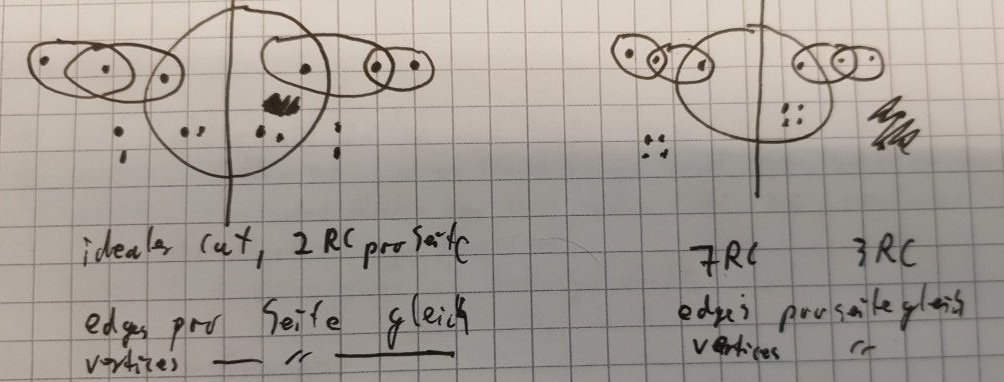
\includegraphics[width=0.65\textwidth]{example.png}
		\caption{Example for a problem with the vertex weight balancing}
	\end{figure}
\end{document}